\section{Introduction}

% TODO Zrobic wstep do wstepu


The documentation is ordered as follows. This sections contains a intuitive overview of Service Architecture Model. Section \ref{sec:samModel} present a precise definition of presented concepts. Abstract Domain Dependency Model defined on section \ref{sec:ioc} is necessary to define service injection. Section \ref{sec:SEE} present a execution model for services of a SAM Architecture.

\subsection{Architecture Overview}

A SAM \textbf{Architecture} defines a \textbf{Service Taxonomy}. Service Taxonomy is a set of separate \textbf{Categories} grouping \textbf{Service Specifications}.

\begin{figure}[h!]
 \centering
 \includegraphics[width=1\textwidth]{taxonomy}
 \caption{Service Taxonomy example}
 \label{fig:taxonomy}
\end{figure}

Figure \ref{fig:taxonomy} shows a service taxonomy consisting of five categories. Each category has different Service Specifications indicated by dots.

% TODO referencja do javy -> zmienic na opis method jako R name(args)
A \textbf{Service Specification} is a set of \textbf{Interfaces}. A Interface intuitively should be treated as a normal Java interface. No class members are allowed on Interfaces. Service Specifications are disjoint.

For one Service Specification it is possible to have many different Service Implementations. A \textbf{Service Implementation} or Implementation is a \textbf{Binding Provider} (see section \ref{sec:ioc}) and all necessary classes to instantiate the Service Specification Interfaces. For simplicity, one can assume that it is a set of classes implementing the Service Specification Interfaces. See \ref{sec:ServiceImplementation} for more details about Service Implementations.

Implementations are executed on a \textbf{Service Execution Environment}. One Implementation executed is called a \textbf{Service Instance} or Instance for short, and it has a unique \textbf{Instance Identificator} (IID). It is possible to execute many Service Instance of the same Service Specification simultaneously. Each Service Instance can be a instantiation of a different Implementation. See section \ref{sec:intSEE} for a overview of Service Execution Environment and section \ref{sec:SEE} for reference information.

To use external services, the Implementation developer must introduce to the code references to interfaces belonging to some external services. \textbf{Dependency Injection Model} is used to inject references to  Service Instances of appropriate type. The choose of  external Service Instance is made completely on the Service Execution Environment as a configuration aspect. The exact definition of Dependency Injection Model is given in section \ref{sec:ioc}.

SAM imposes constraints on the external services used in Implementations defined be a \textbf{Category Accessibility Relation}:  category $C_2$ is accessible to category $C_1$ if we allow injection of interface of services from category $C_2$ in the implementation of services of $C_1$. As an example, assume that category accessibility relation for architecture given in figure \ref{fig:taxonomy} is as follow:
\begin{eqnarray}
\text{User Services} &\hookleftarrow & \text{Core Services} \nonumber \\
\text{Core Services} &\hookleftarrow& \text{Core Services} \nonumber \\
\text{Core Services} &\hookleftarrow& \text{Infrastructure Services} \nonumber \\
\text{Core Services} &\hookleftarrow& \text{Management Services} \nonumber \\
\text{Core Services} &\hookleftarrow& \text{Information Services} \nonumber 
\end{eqnarray}

This mean that a Service Implementations of Service Specification belonging to Category ``User Services'' can inject only references to Service Instances belonging Category ``Core Service''.

\subsection{Service Specification}

We present on more detailed overview of Service Specification definition and some concrete examples.

% TODO cambiar el nombre del service
Lets see the definition of ``UserData'' Service Specification belonging to Category ``User Service''. It is defined be two interface's as shown on listing \ref{UserServiceSimple},\ref{UserServiceComplex}.

\lstinputlisting[label=UserServiceSimple,caption=Service Specification Interface API - UserData]{../srcAPI/eu/pmsoft/sam/service/user/UserDataSimpleAPI.java}

Method \lstinline|simpleMethod| is just a simple example without arguments and return type \lstinline|boolean|. Method \lstinline|complexInteractionAPI| is more interesting, it has a simple type argument and returns a reference to interface \lstinline|UserDataComplexAPI| defined below. On SAM Interface methods signature it is allowed to use only primitive types and interface types declared on the architecture.

A important relation between Interfaces is the \textbf{Signature Relation} resulting from the types used on methods signatures. As a examples we say that Interface \lstinline|UserDataSimpleAPI| uses Type related to \lstinline|UserDataComplexAPI| because it appears as a return type of method \lstinline|complexInteractionAPI|. Please note that Signature Relation is defined between Interfaces and Types resulting from Interfaces.

\lstinputlisting[label=UserServiceComplex,caption=Service Specification Interface API - UserData]{../srcAPI/eu/pmsoft/sam/service/user/UserDataComplexAPI.java}

Interface \lstinline|UserDataComplexAPI| is very similar to previous one. It defines three methods with some parameters and result types. Note that there are two new interfaces \lstinline|DomainData| and \lstinline|DomainTypeExample| not belonging to the Service Specification. A set of interfaces used on a Service Specification is called a \textbf{Domain Specification}. It is required for Domain Specifications to be mutually disjoint.

% , shown on listing \ref{DomainData},\ref{DomainTypeExample}
% \lstinputlisting[label=DomainData,caption=DomainData Interface]{../srcAPI/eu/pmsoft/sam/ds/DomainData.java}
% \lstinputlisting[label=DomainTypeExample,caption=DomainTypeExample Interface]{../srcAPI/eu/pmsoft/sam/ds/DomainTypeExample.java}

Signature Relation implies a \textbf{Domain Dependency Relation} between Domain Specifications: If a type derived from Domain Specification $d_2$ is used on some method signature of a Interface from Domain Specification $d_1$, then we say that $d_1$ depends on $d_2$.

We treat Service Specification as a Domain Specification, but do not allow to use Types from Service Specifications on other Domain Specifications. We also require that the Domain Dependency Relation be acyclic. A possible graph related to a Domain Dependency Relation is shown on figure \ref{fig:service}.

\begin{figure}[ht!]
 \centering
 \includegraphics[width=1\textwidth]{serviceSpec}
 \caption{Domain Dependency Relation example}
 \label{fig:service}
\end{figure}

A Domain Specification without dependencies is called a Simple Domain Specification. If it has dependencies, then is called Model Domain Specification. As mentioned earlier, a Service Specification can't be used as a dependency.



Lets define a Service Specification ``CoreServiceExample'' containing interface \ref{CoreServiceExample} to be used in the following examples.

\lstinputlisting[label=CoreServiceExample,caption=CoreServiceExample Service Specification]{../srcAPI/eu/pmsoft/sam/service/core/CoreServiceExample.java}


\subsection{Service Implementation and Service Instance Injection}
\label{sec:ServiceImplementation}

A simple implementation ONE of Service Specification ``CoreServiceExample'' is class \lstinline|ImplementationCoreServiceExampleOne| implementing interface \lstinline|CoreServiceExample|, see listing \ref{ImplementationCoreServiceExampleOne}.

\lstinputlisting[label=ImplementationCoreServiceExampleOne,caption=Implementation ONE of ``CoreServiceExample'']{../srcAPI/eu/pmsoft/sam/impl/core/ImplementationCoreServiceExampleOne.java}

Note fields of Type \lstinline|CoreServiceExample|. These are examples of \textbf{Injection Points}, places where it is possible to receive injections, it is references to external Service Instance. Field \lstinline|public CoreServiceExample serviceInjectionPointWithBindingAnnotation;| has also a Binding Annotation. \textbf{Binding Annotations} instruct the Service Execution Environment on how to interconnect Service Instances. Each Injection Point has associated a \textbf{Key} defined as a pair Type-Binding Annotation. Binding Annotation may be empty.

A Implementation TWO of ``CoreServiceExample'' is created with classes \lstinline|ImplCoreTwo|,\lstinline|ImplCoreTwoBinding| and a non trivial Binding Provider following scheme:
\begin{eqnarray}
\text{CoreServiceExample}\times 0 &\longmapsto& \text{ImplCoreTwo} \nonumber \\
\text{CoreServiceExample}\times\text{@BindingAnnotationExample} &\longmapsto& \text{ImplCoreTwoBinding} \nonumber 
\end{eqnarray}
Implementation TWO provides a different class implementing \lstinline|CoreServiceExample| according to used Key.

Assume that on the Service Execution Environment are created two Instances of Service Specification ``CoreServiceExample'' using previously presented Implementations ONE and TWO, with IID ``01'' and ``02'' respectively.

Service Execution Environment could be configured to inject Instance ``02'' to Instance ``01'' as shown in figure \ref{fig:instanceinjection01}.

\begin{figure}[h!]
 \centering
 \includegraphics[width=1\textwidth]{instanceInjection01}
 \caption{Service Instance injection}
 \label{fig:instanceinjection01}
\end{figure}

Other possible scenario is to inject Instance ``01'' on Instance ``01'' as shown on figure \ref{fig:instanceinjection02}. Implementation ONE don't define any binding for key $\text{CoreServiceExample}\times \text{@BindingAnnotationExample}$, so the simplest key $\text{CoreServiceExample}\times 0$ is used because it also match the annotated Injection Point.

\begin{figure}[h!]
 \centering
 \includegraphics[width=1\textwidth]{instanceInjection02}
 \caption{Self-Reference injection}
 \label{fig:instanceinjection02}
\end{figure}

For details on Dependency Injection Model and Injection Process see section \ref{sec:ioc}.

\subsection{Service interaction and Canonical Execution Protocol}
\label{sec:intCallProtocol}

Existing service interaction methods and technologies are based on a function execution abstraction, a service is understood as a external set of functions available through remote calls. This approach leads to the following logical scheme during architecture and software development:
\begin{itemize}
 \item Prepare service request data
 \item Execution: Send service request, wait for response
 \item Interpret response
\end{itemize}
Such a pattern is associated with high costs related to calls on external service. This leads to creation of increasingly complex data structures to define the parameters and results of service methods, or ``external functions''.

SAM introduce a completely new approach to service calls and service interaction. To illustrate this,  lets use a Implementation of ``UserData'' Service Specification that contain class \lstinline|ImplementationOneSimple| shown on listing \ref{ImplementationOneSimple}.
% ,\ref{ImplementationOneComplex}.
% and \lstinline|ImplementationOneComplex|

\lstinputlisting[label=ImplementationOneSimple,caption=Class of UserData Implementation]{../srcAPI/eu/pmsoft/sam/impl/user/one/ImplementationOneSimple.java}

Method \lstinline|public boolean simpleMethod()| is implemented using external service ``CoreServiceExample''. Note that executing this method may require a large number of calls to interface \lstinline|CoreServiceExample|, but how many external requests are needed? only one!. See listing \ref{CoreServiceExample} for the definition of interface \lstinline|CoreServiceExample| and note that only the \lstinline|isProcessStatusOk| method has a return type different that \lstinline|void|. SAM define a \textbf{Canonical Execution Protocol} to serialize calls to Service Specification Interfaces. Execution of method \lstinline|public boolean simpleMethod()| serialized with the canonical protocol produce a service request containing:
\begin{verbatim}
i_0.resetProcess()|i_0.putData(i_1)|...
...i_0.putData(i_n)|i_0.isProcessStatusOk()r_0|
PAYLOAD
i_0=KEY<CoreServiceExample X 0>
i_1="IntegerSerialization"
...
i_n="IntegerSerialization"
r_0=Type<boolean>
\end{verbatim}

This is the exact information necessary for a external Service Instance implementing ``CoreServiceExample'' to repeat calls to interface \lstinline|CoreServiceExample| and return the final result.



Generally, an external call is required when the return type of a Interface method is a class type. In the case that a return type is a interface type, it is possible to continue ``recording'' executions to that interface without any external request. See method \lstinline|changeUserName| on listing \ref{CanonicalWithInterface} and resulting canonical service request.

\lstinputlisting[label=CanonicalWithInterface,caption=Calls to external service with nested interface executions]{../srcAPI/eu/pmsoft/sam/examples/ServiceCode.java}

\begin{verbatim}
i_0.sendData(i_1)r_0|r_0.sendMoreData(i_2)r_1|
PAYLOAD
i_0=KEY<ExternalServiceInterface X @BindingAnnotationExample>
r_0=InterfaceType<NestedExternalInterface>
i_1="IntegerSerialization"
i_2="StringSerialization"
r_1=Type<Boolean>
\end{verbatim}
In this case also, only one external request is necessary to realize service interaction.

The reason for which Domain Specifications consist only of interfaces is to maximize the possible sequences of calls without exchange of requests between Service Instances.

\subsection{Service Implementation development}
\label{sec:intImpleDEVEL}



A Service Implementation that don't inject any external Service is called a \textbf{Prototype Implementation} or Prototype. During development of any Service Implementation, it is very convenient to have Prototypes for each used Service Specification. If a Prototype implementation of each used Service Specification is available, then a local execution environment can be easily created.


Having Prototypes injected it is possible to execute internal tests. A SAM Architecture can additionally provide predefined tests for a given Service Specification called Test Specification. \textbf{Test Specification} is a set of test classes containing injection points only for one given Service Specification. Note that Test Specifications can be developed independently of any Service Implementations.The use of Canonical Execution Protocol for service interaction makes possible to create Test Specification on base of previously recorded services interaction. In case that a complex bug is found on some Implementation, a test case could be recorded and then executed on all existing Implementations.

Using Prototypes and Test Specifications on development process leads to Service implementations with defined injection as in figure \ref{fig:serviceImplementation}.

\begin{figure}
 \centering
 \includegraphics[width=1\textwidth]{serviceImplementation}
 \caption{Service Implementation injection for development}
 \label{fig:serviceImplementation}
\end{figure}

\newpage
\subsection{Service Execution Environment}
\label{sec:intSEE}

Execution of a Service Implementation to create Service Instances is done by injecting dependencies for some existing Service Instance. Injection Process defined on section \ref{sec:iocIP} support such execution process, allowing also the creation of cyclic injections between Service Instance. Each Service Instance gets a unique Instance ID (IID).

\textbf{Injection Configuration} defining Service Instance injection is a mapping
\begin{eqnarray}\label{sseconfig}
config: IID \times Service Specification \longrightarrow IID \nonumber
\end{eqnarray}
maintained by a \textbf{Service Execution Environment}.

Note that Service Implementations don't have any control over the injection process, they don't even have knowledge of IID of injected Service Instances. All the control over Service Instance injection is transferred to the Service Execution Environment.

Given two Injection Configurations, it is possible to merge then in a new mapping. This ensure Service Execution Environment scalability.

Two Service Execution Environments not trusting each other, can share limited information about running Services Instances and enable service interaction under the supervision of special security policies.





